\section{Projektafgrænsning}
Semesterprojektet afgrænses til at have fokus på grafiske brugergrænseflader (\gls{pcapp}, samt \gls{iosapp}), datakommunikation og database design. Projektet har altså fokus på softwaredelen af \gls{smartpool} og ikke elektronik delen.

Brugeren skal kunne oprette en profil/bruger i \glspl{smartpool} \gls{pcapp} og registrere sit produkt. \gls{smartpool} systemet og dets grafiske brugerflader bør nu kunne tilgå databasen. \gls{smartpool} overholder da læringsmålene til semesterprojektet, fordi grafisk brugerflade, netværkskommunikation og databaser indgår.

\begin{figure}
	\centering
	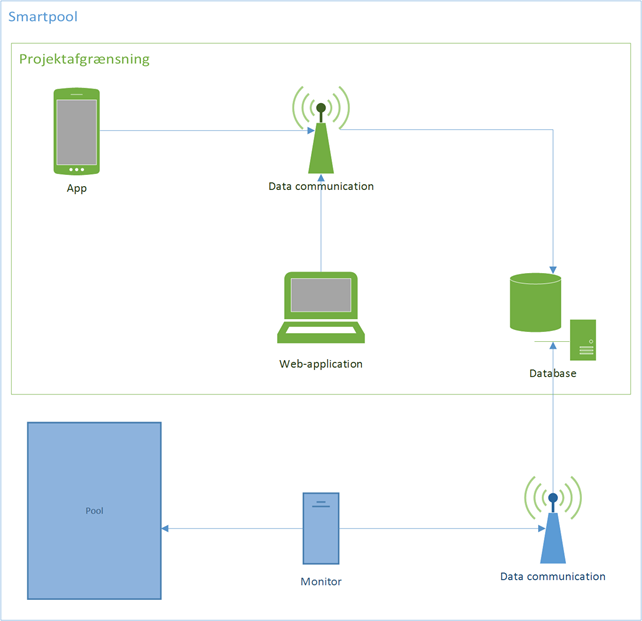
\includegraphics[width=0.9\linewidth]{figs/afgraensning.png}
	\caption{Projektet vil omhandle indholdet i den grønne indramning.}
	\label{fig:afgraensning}
\end{figure}
\todo{Figur skal mulighed ændres lidt så det er klart at vi også laver et PC program.}